\chapter{Experiments}
\label{chp:experiments}

The \rrtfunnel{} algorithm developed this far will now be tested in a simulation
experiment where a simple unicycle model of a car will be set to traverse a
small strip of forest. The simulation environment can be seen in
figure~\cref{fig:simulated-forest}, where the vehicle starts at one end of the
obstacle forest, and is set to traverse the strip of forest and reach any
\((x,y)\) position in a circle of radius five surrounding the endpoint thirty
five meters ahead.

\begin{figure}
  \centering 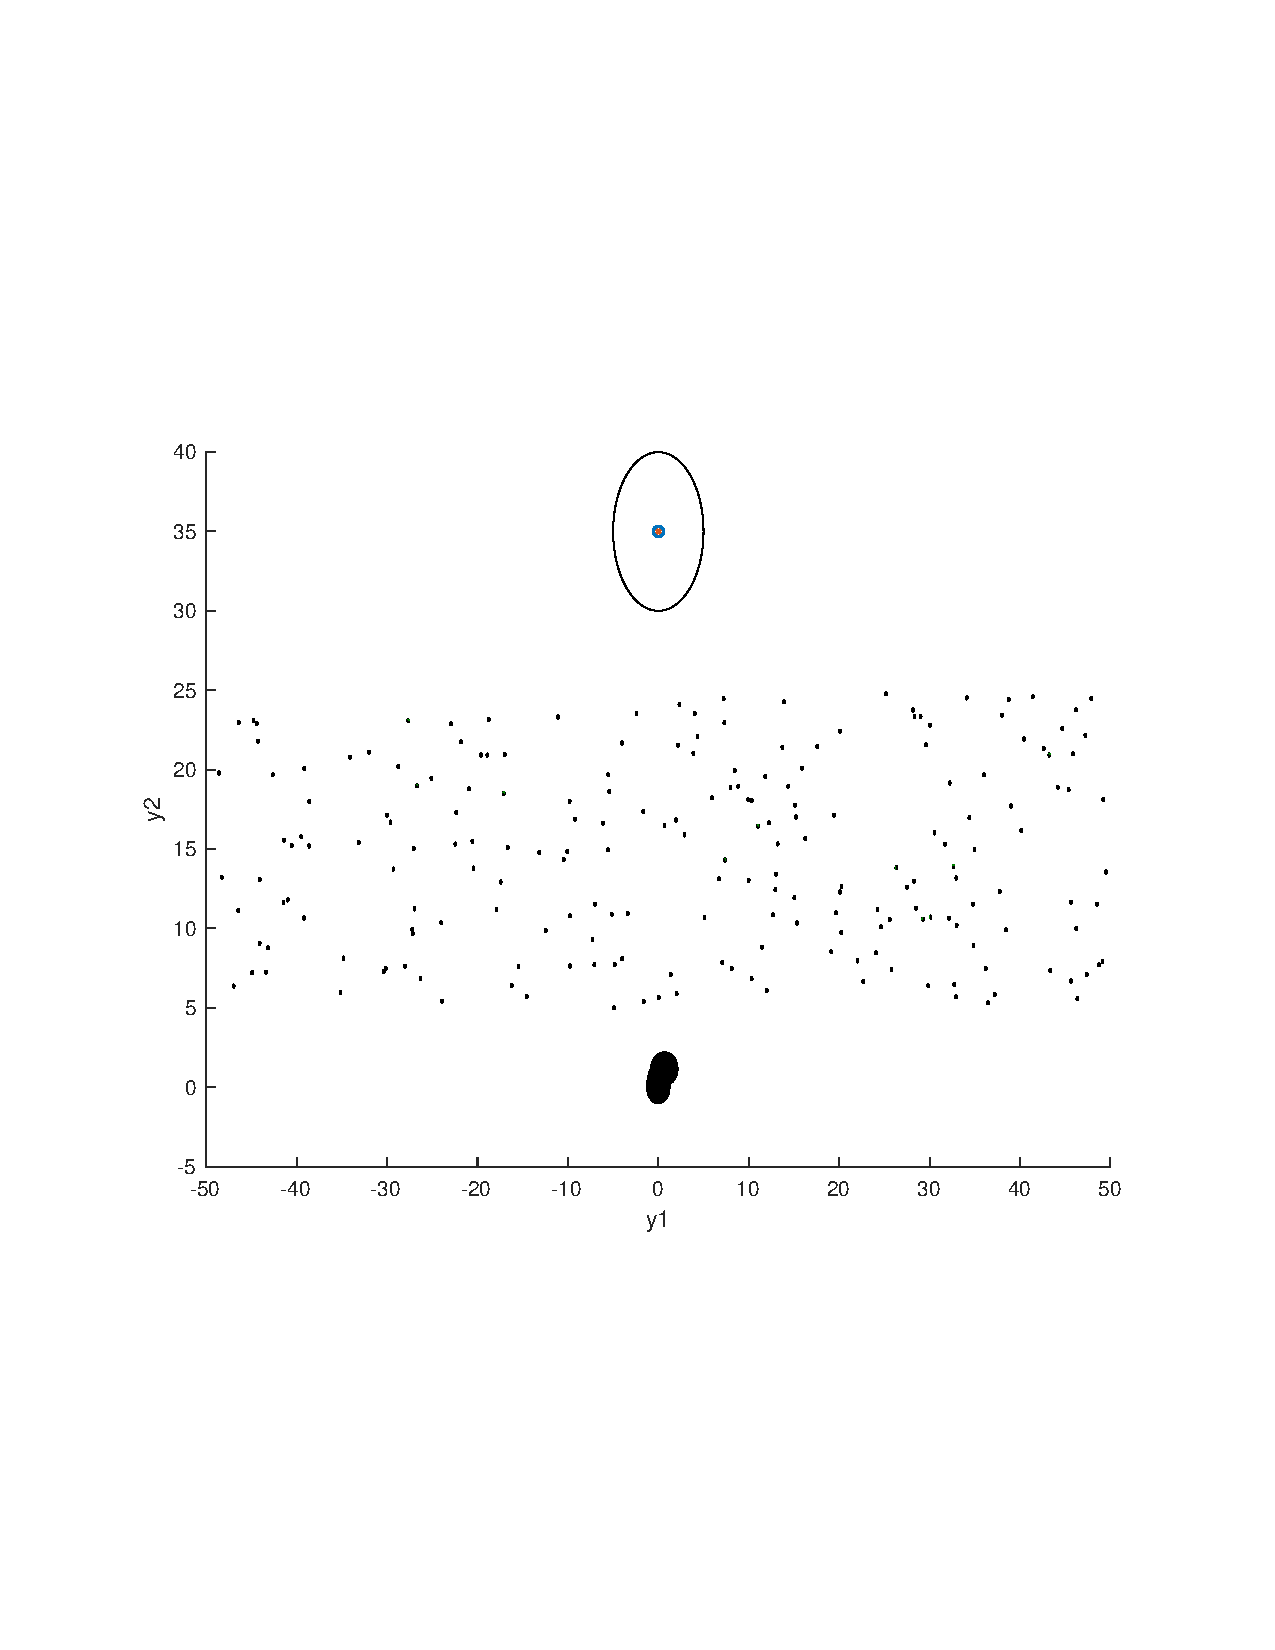
\includegraphics[scale=.5]{figures/experiments/simulated-forest}
  \caption{The experiment environment.}
  \label{fig:simulated-forest}
\end{figure}

\section{Testing the \rrtfunnel{} algorithm}

The experiment section starts out by generating a random strip of forest for
which the airplane has to navigate through in \cref{sec:Poisson-Process}. Next
it expands from the single point model in \cref{eq:dynamical-model} to
incorporate the actual size of the model in \cref{subsec:deciding-model-size},
and then shows how to expand the size of the funnels to incorporate the expanded
model in \cref{subsec:expand-funnel}. It then continues to show the initial
motion primitive set and the \ac{LQR} controller weightings in
\cref{subsec:initial-motion-primitive,subsec:lqr-cost}. It then shows how a
\textit{Monte-Carlo} simulation is run in order to make sure that the expanded
model actually stays within the expaned funnels in
\cref{subsec:check-vehicle-in-funnel}, and shows that the funnel composition
guarantees are lost due to the data shown in \cref{subsec:funnel-no-composable},
until finally presenting the results of the \rrtfunnel{} algorithm benchmarked
against a conservative \ac{RRT} motion planner which does not handle the
uncertainty that is provided by the cross-wind in \cref{sec:experiments-final}.

\subsection{Generating the obstacle forest (Poisson processes)}
\label{sec:Poisson-Process}

In order to generate the obstacle field for the experiments, which is to
resemble a forest, a \textit{spatial Poisson process} is employed. Poisson
processes are used to model random configurations of points in
space'~\cite{Kroese_2014}, and hence are well suited for generating a simulated
forest. For the experiments below, a forest will be the realization of a spatial
Poisson process on \(\R^2\).

A few key parameters of the Poisson process has to be set for use in the
experiments below. Firstly, \(\lambda\) is the intensity of the spatial process.
For these experiments, the intensity will be held constant, and the process is
therefore homogeneous, as it does not vary with the position in space. One
interesting configuration could be to vary the intensity as the radius from
origo, and hence the difficulty in traversing the terrain would increase with
the distance traveled. However, the constant intensity setting was chosen to
keep things simple and uniform.

The algorithm for realizing a random Poisson measure~\cref{def:Poisson-def} is
taken from~\cite[Definition 1.1.1,p~34]{Kroese_2014}.

\begin{definition}[Generating a Poisson random measure]
  \label{def:Poisson-def}
  \begin{enumerate}
  \item Generate a Poisson random variable \(N \sim Poi(\mu(E))\).
  \item Draw \(X_1,X_2,\ldots,X_N \sim g\), where \(g(x) \lambda(x)/ \mu(E)\).
  \end{enumerate}
\end{definition}
where \(E\) is the set over which the points should be generated, and the
\textit{pdf} \(g(x_1, x_2) = \lambda(x)/\mu(E)\). Finally, \(\mu(E)\) is defined
as
\[
  \mu(E) = \int_{E} \lambda(x) dx.
\]

For the experiments the set \(E\) will be a square defined as
\[
  E = {[-\alpha, \alpha]}^2
\]
the density of the generated forest \(\lambda\) will be set to
\[
  \lambda = 0.1
\]
of which the resultant forest on a \(20 \times 20\) grid can be seen in
figure~\cref{fig:poisson009}.

\begin{figure}
  \begin{subfigure}[b]{0.5\textwidth}
    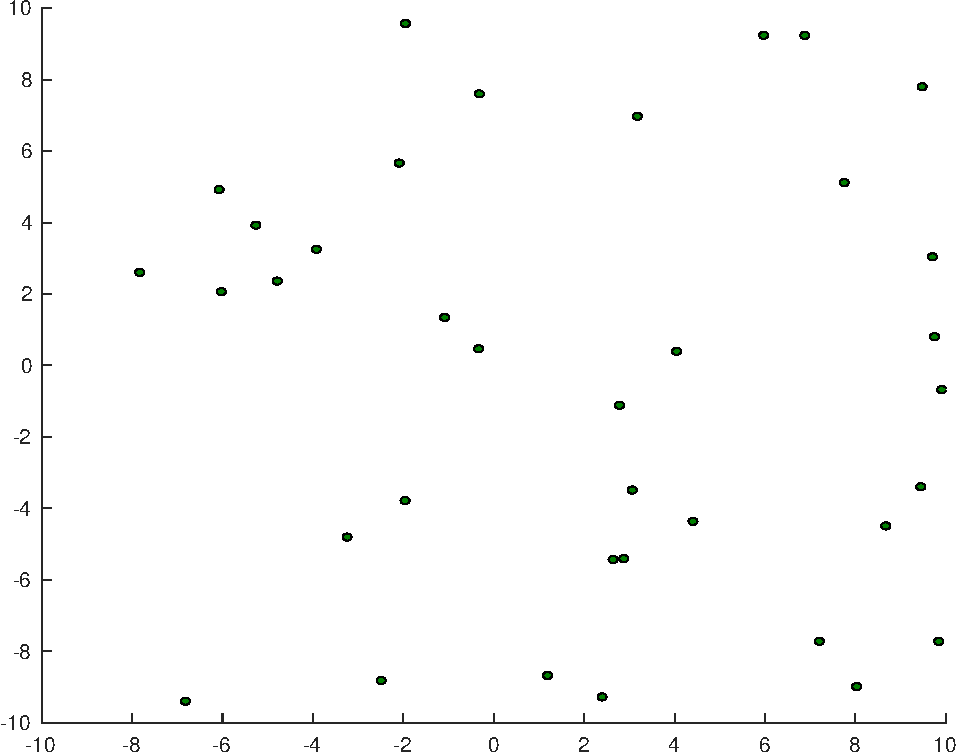
\includegraphics[width=\textwidth]{figures/experiments/poisson009}
    \caption{The resultant forest generated by a spatial Poisson process with
      intensity \(\lambda = 0.1\)}
    \label{fig:poisson009}
  \end{subfigure}%
  \begin{subfigure}[b]{0.5\textwidth}
    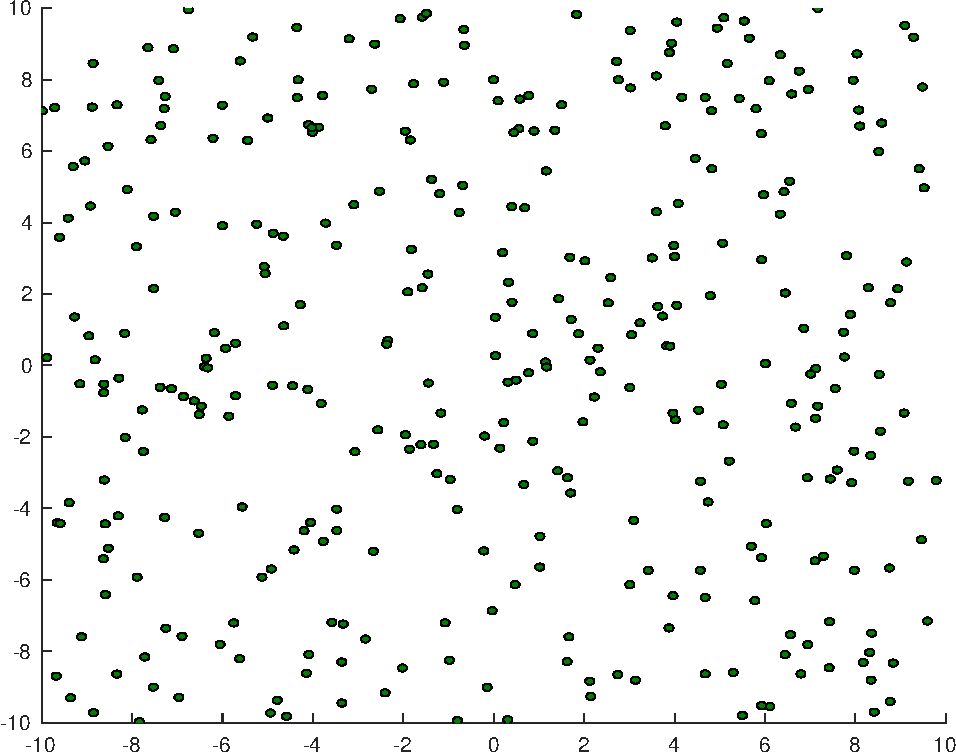
\includegraphics[width=\textwidth]{figures/experiments/poisson09}
    \caption{The resultant forest generated by a spatial Poisson process with
      intensity \(\lambda = 0.9\)}
    \label{fig:poisson09}
  \end{subfigure}
\end{figure}

\subsection{Deciding upon the size of the vehicle and the obstacles}
\label{subsec:deciding-model-size}

The funnels generated thus far is created from a point model of the vehicle, and
its dynamics. If the grid that the simulations are run on are set to have an
increment of a meter, then the funnels from the basic set are given a velocity
of \([v(t)] = \si{m.s^{-1}}\), \([\theta] = \si{\radian\per\second}\), and
\([\dot{\theta}] = \si{\radian\per\second\per\second}\), where \([\cdot]\) is
the unit operator. The size of the vehicle is arbitrary, and can be chosen
freely, but if it is imagined as a radio controlled car, with a speed of
\(10\si{m.s^{-1}}\), then a size of \(30 \times 20 \si{\centi\metre} \) keeps
everything within the realm of a normal radio controlled car and its
capabilities. The mass is not relevant for our first order dynamics, but still
the vehicle is assigned a mass of \(1 \si{\kilo}\), so that the translation of
the model dynamics is not irrelevant. A figure of the vehicle can be seen in
figure~\cref{fig:radio-vehicle}.

\begin{figure}
  \centering 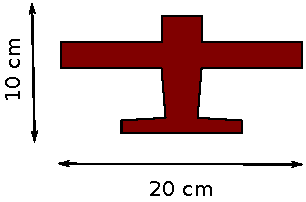
\includegraphics[trim={5cm 5cm 5cm 5cm},
  width=\textwidth]{figures/experiments/radio-vehicle-model}
  \caption{The airplane employed in the simulation experiments.}
  \label{fig:radio-vehicle}
\end{figure}

\subsection{Expanding the size of the funnel by the size of the simulated
  vehicle}
\label{subsec:expand-funnel}

The size of the vehicle in the original model is a single point, and as such,
the vehicle model with a size is not accounted for in the funnels prior to
running the simulations. Therefore the funnels have to be expanded in order for
them to accommodate the necessary robustness guarantees that are expected from
the algorithm. However, the size of the vehicle only affects the size of the
funnel ellipsis projected down into the xy-plane. Therefore first getting the
projected size of the funnel, where \(P \colon \R^4 \rightarrow \R^2\) is a
projection map with a projection matrix
\[
  P =
  \begin{bmatrix}
    I_{2 \times 2} & \mathbf{0}_{2 \times 2} \\
  \end{bmatrix}
\]
such that for the projected ellipsoid
\[
  \mathcal{E}_{p} = \set{\bar{x} \in \R^{2} \mid {\bar{x}}^{T}S_{k}^{(p)}\bar{x}
    \leq 1}
\]
and
\[
  S_{k}^{(p)} = {\left( PS_{k}^{-1}P^T \right)}^{-1}
\]
and \(\mathcal{E}_{p}\) is the projected set of the ellipsoid projected down
into the xy-plane~\cite{majumdarFunnelLibrariesRealtime2017}. In general an
ellipse centered at the origin is a linear transformation of the unit
circle~\cite{lay2005linear}. Exploiting this fact, expanding the radius of the
circle to encompass the vehicle model. Also taking into account that the matrix
\(S_{k}\) is \textit{Positive semidefinite}, and hence can be Cholezky
factorized~\cite{lay2005linear}. The expanded ellipsis (which now contains all
the possible states of the vehicle model) is:

\begin{align*}
  S_{k}^{\mathcal{P}} &= R^{T}R \\
  \mathcal{C} &= \set{y \in \R^2 \mid y^{T}y \leq 1 + r_{vehicle}} \\
  S_{k}^{p'} &= R^{-1}y \\
\end{align*}

where \(S_{k}^{'}\) is the ellipsoid which contains the volume of the vehicle
for all verified states in the funnel. A picture of the initial funnel and the
funnel expanded around the vehicle model can be seen in
figure~\cref{fig:expanded-funnel,fig:expanded-and-unexpanded}.

\begin{figure}
  \centering 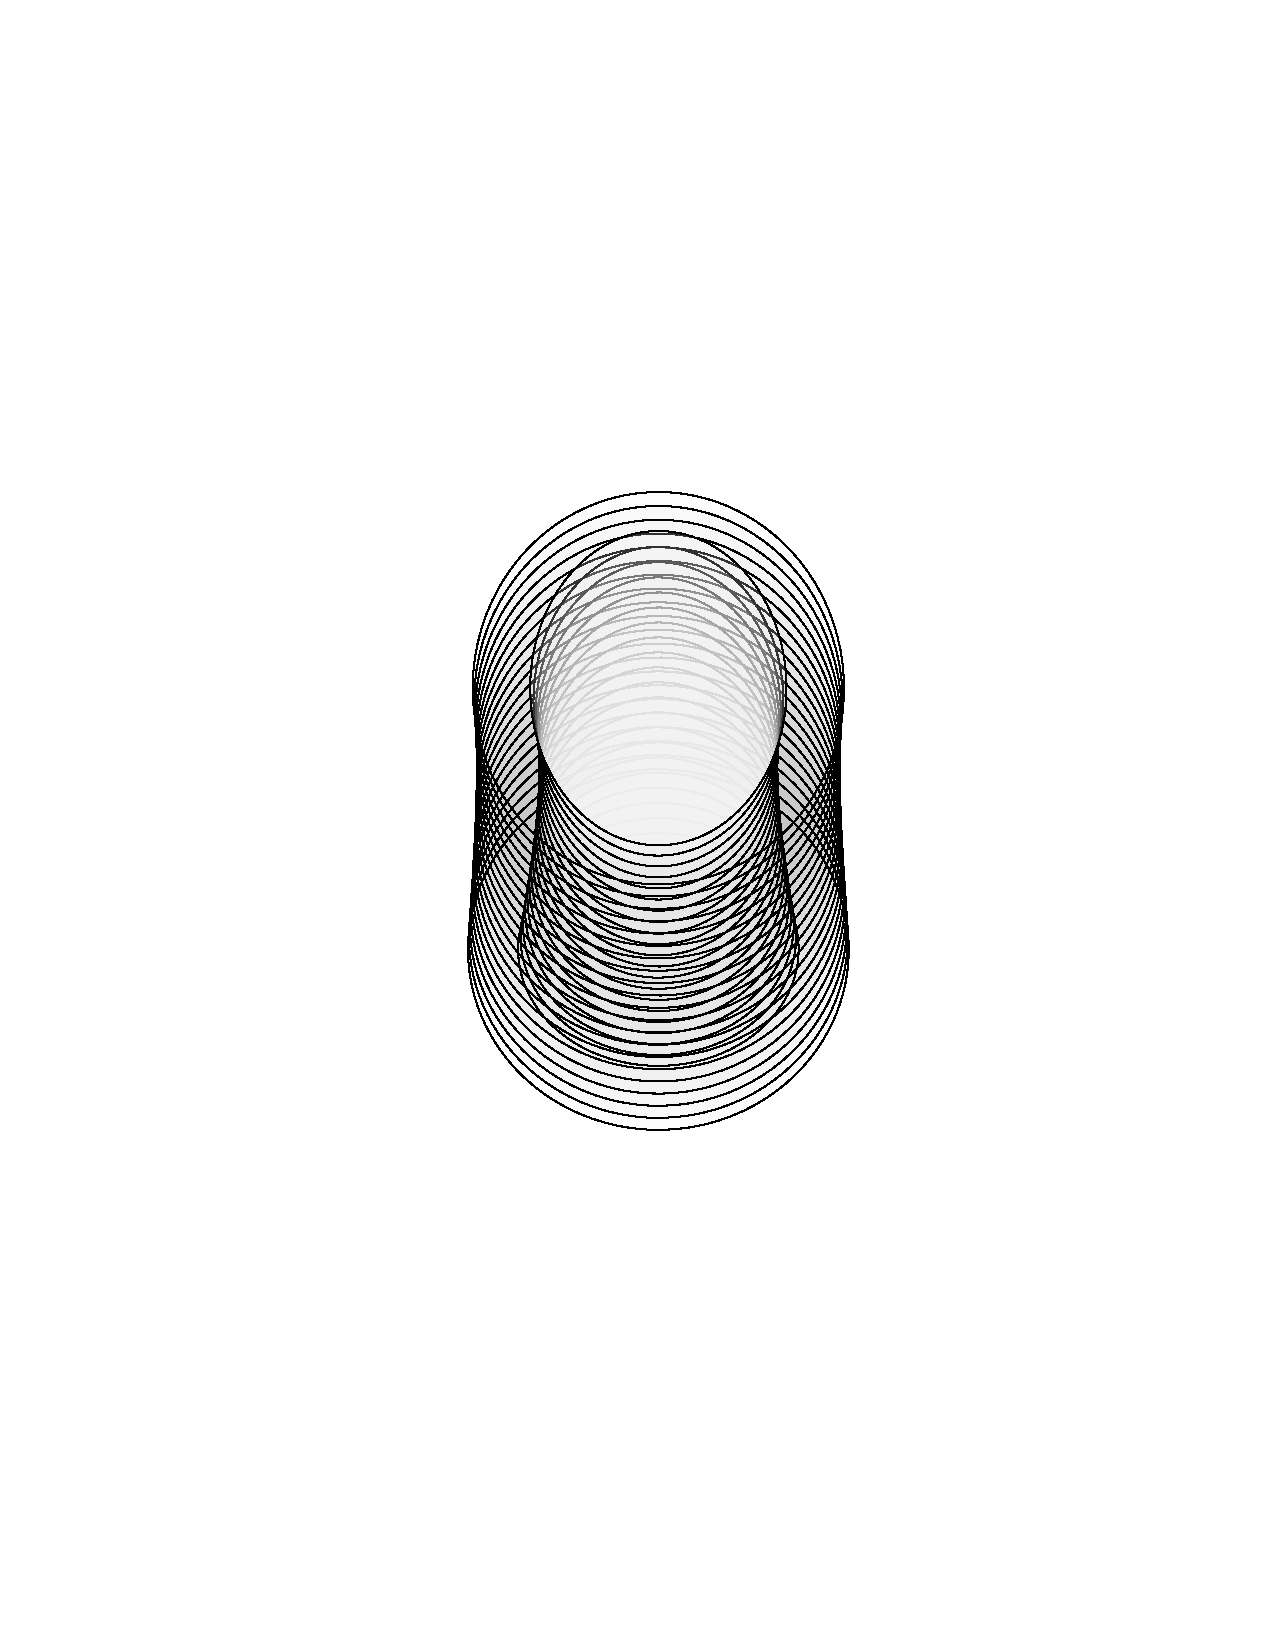
\includegraphics[clip, trim=6cm 8cm 6cm 8cm,
  scale=.5]{figures/method/expanded-funnel}
  \caption{The original funnel created from the point model, with a funnel
    expanded by a radius of 0.1 surrounding it.}
  \label{fig:expanded-funnel}
\end{figure}

\begin{figure}
  \begin{subfigure}{0.5\textwidth}
    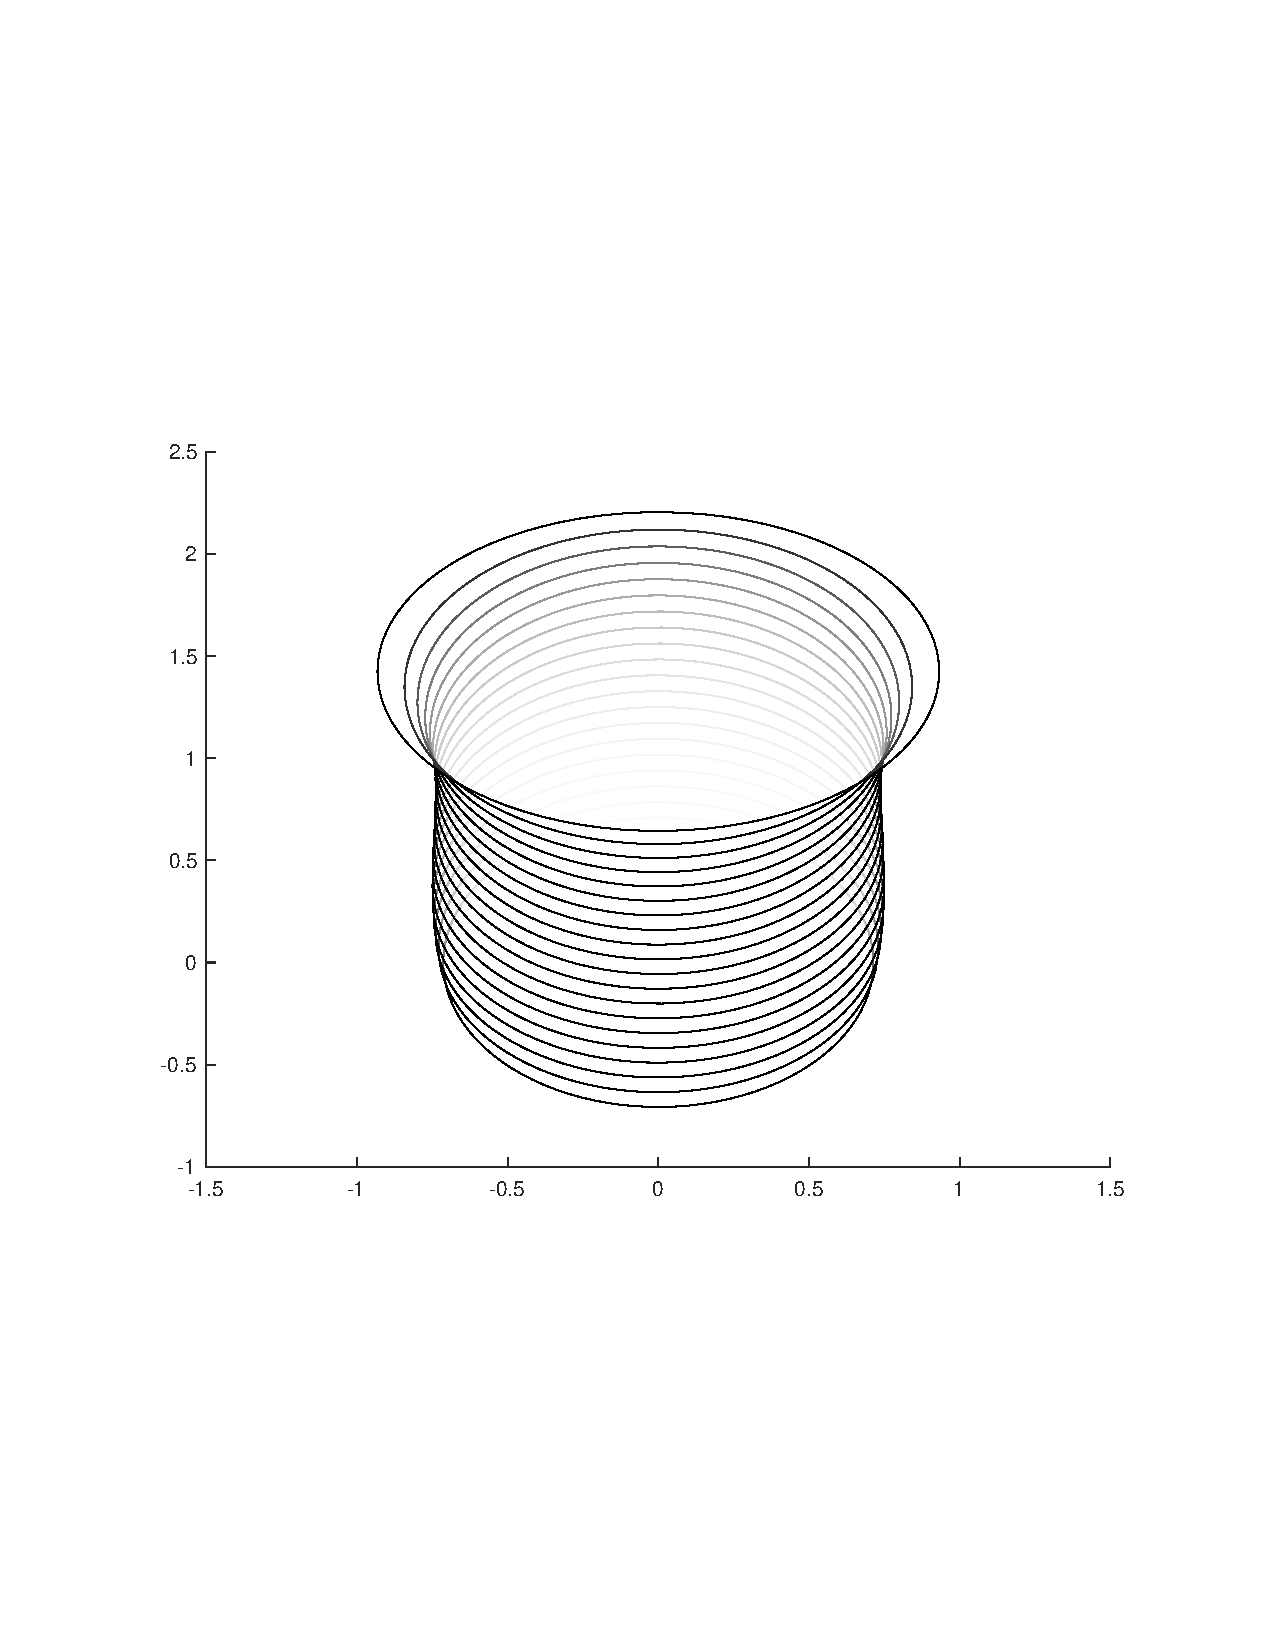
\includegraphics[trim={2cm 5cm 0cm 5cm},
    width=\textwidth]{figures/experiments/unexpanded-funnel}
    \caption{The funnel around a straight trajectory for the point
      model.\newline}
  \end{subfigure}%
  \;
  \begin{subfigure}{0.5\textwidth}
    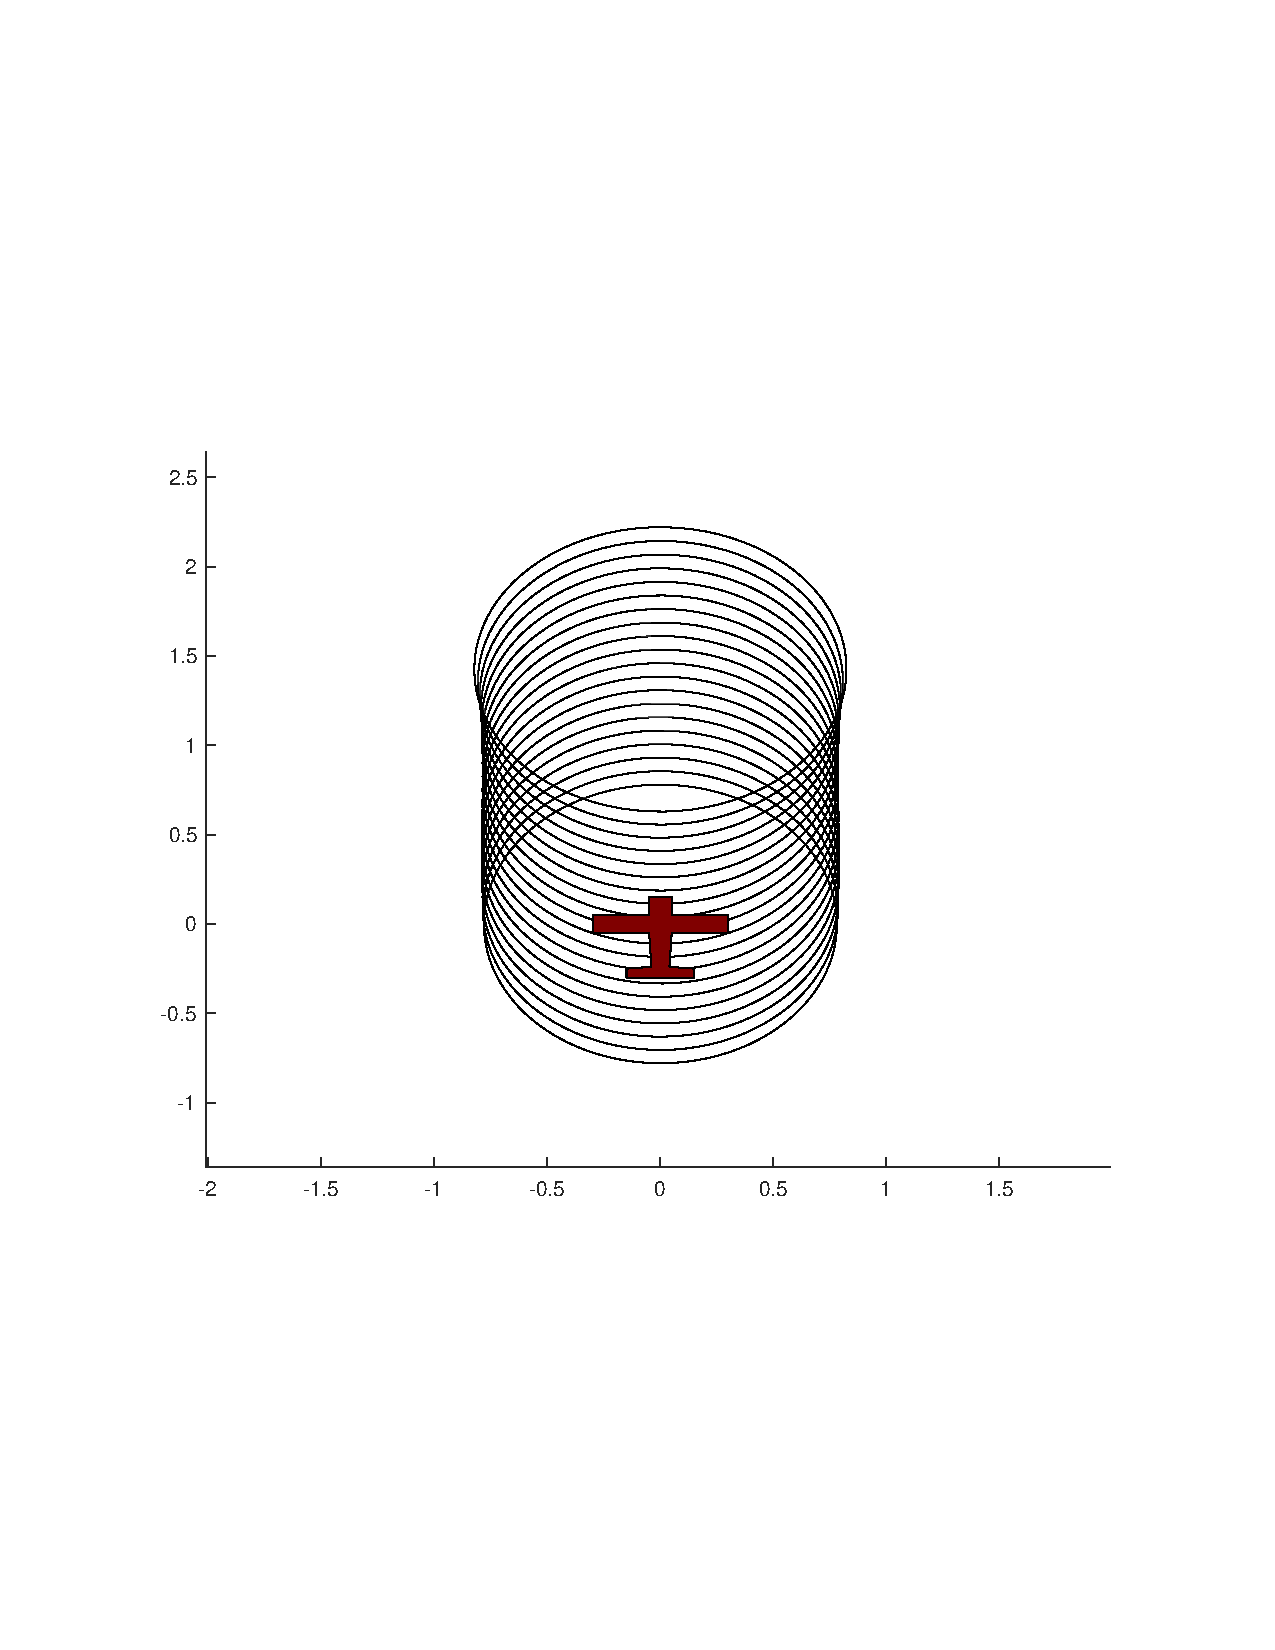
\includegraphics[trim={2cm 5cm 0cm 5cm},
    width=\textwidth]{figures/experiments/expanded-funnel-with-plane}
    \caption{The funnel around a straight trajectory for the point model,
      expanded with the size of the plane.}
  \end{subfigure}
  \caption{Pictured: An unexpanded and a funnel expanded by the size of the
    simulation plane.}
  \label{fig:expanded-and-unexpanded}
\end{figure}

\subsection{The initial motion primitive set}
\label{subsec:initial-motion-primitive}

The basis set of motion primitives should be small, yet cover enough of the
finer movements of the vehicle so that the motion of the vehicle can be near
continuous when composed together. Thus in order to generate a `dense' set of
motion primitives the~\cref{alg:initial-motion-primitives-generation} is
employed to generate points along the arch of a circle with \(N\) different
radii.

\begin{algorithm}[H]
  \label{alg:initial-motion-primitives-generation}
  \caption{Generating the initial motion primitives (TODO) - update with the new
    primitives!}
  \DontPrintSemicolon \SetAlgoNoLine

  \KwIn{%
    \(n\) - Number of points along the arch \\
    \(r_{0}\) - Initial radius \\
    \(r_{f}\) - Final radius \\
    \(s\) - Step-size (\(r_{n+1} = r_{n} + s\)) } \KwOut{\(\mathbf{X}\) -
    Endpoints matrix for the trajectory generator}

  \(\theta_{0} = \pi\) \;

  \For{\(r_{k+1} = r_{k} + s\)}{ \(\theta_{j} = \frac{\theta{0}}{2r}\) \;
    \(\theta_{stepsize} = \frac{\theta{j}}{(n-1)/2}\) \; \(\mathbf{X} \leftarrow
    (r_{k+1}, \theta=0)\) \; \For{\(i = 1 \) \KwTo \(\frac{n-1}{2}\)}{
      \(\theta_{ki} = i*\theta_{stepsize}\) \; \(\mathbf{X} \leftarrow (r, \pm
      \theta_{ki})\) \; }\; }\;
\end{algorithm}

The initial trajectories employed in the experiments can be seen
in~\cref{fig:intial-trajectories-exp}, and the projected funnels overlaid a
sample in~\cref{fig:sample-funnel-overlay}.

\begin{figure}
  \centering
  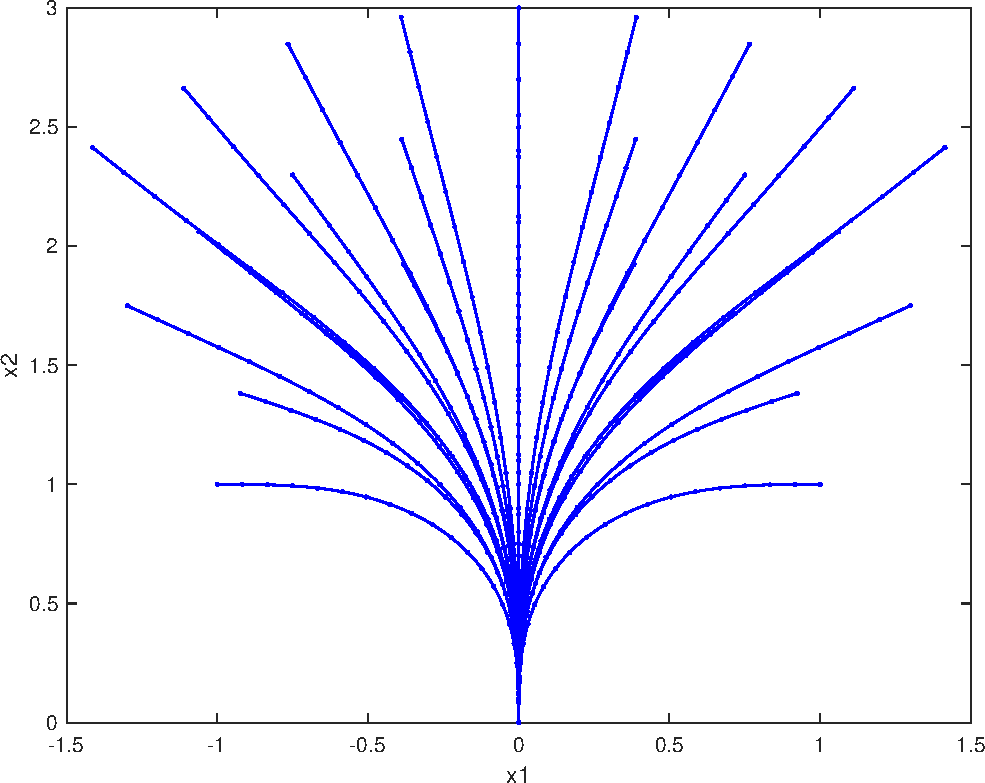
\includegraphics[scale=.5]{figures/experiments/initial-trajectories}
  \caption{The initial trajectories used in the \rrtfunnel{} algorithm.}
  \label{fig:intial-trajectories-exp}
\end{figure}

\begin{figure}
  \centering
  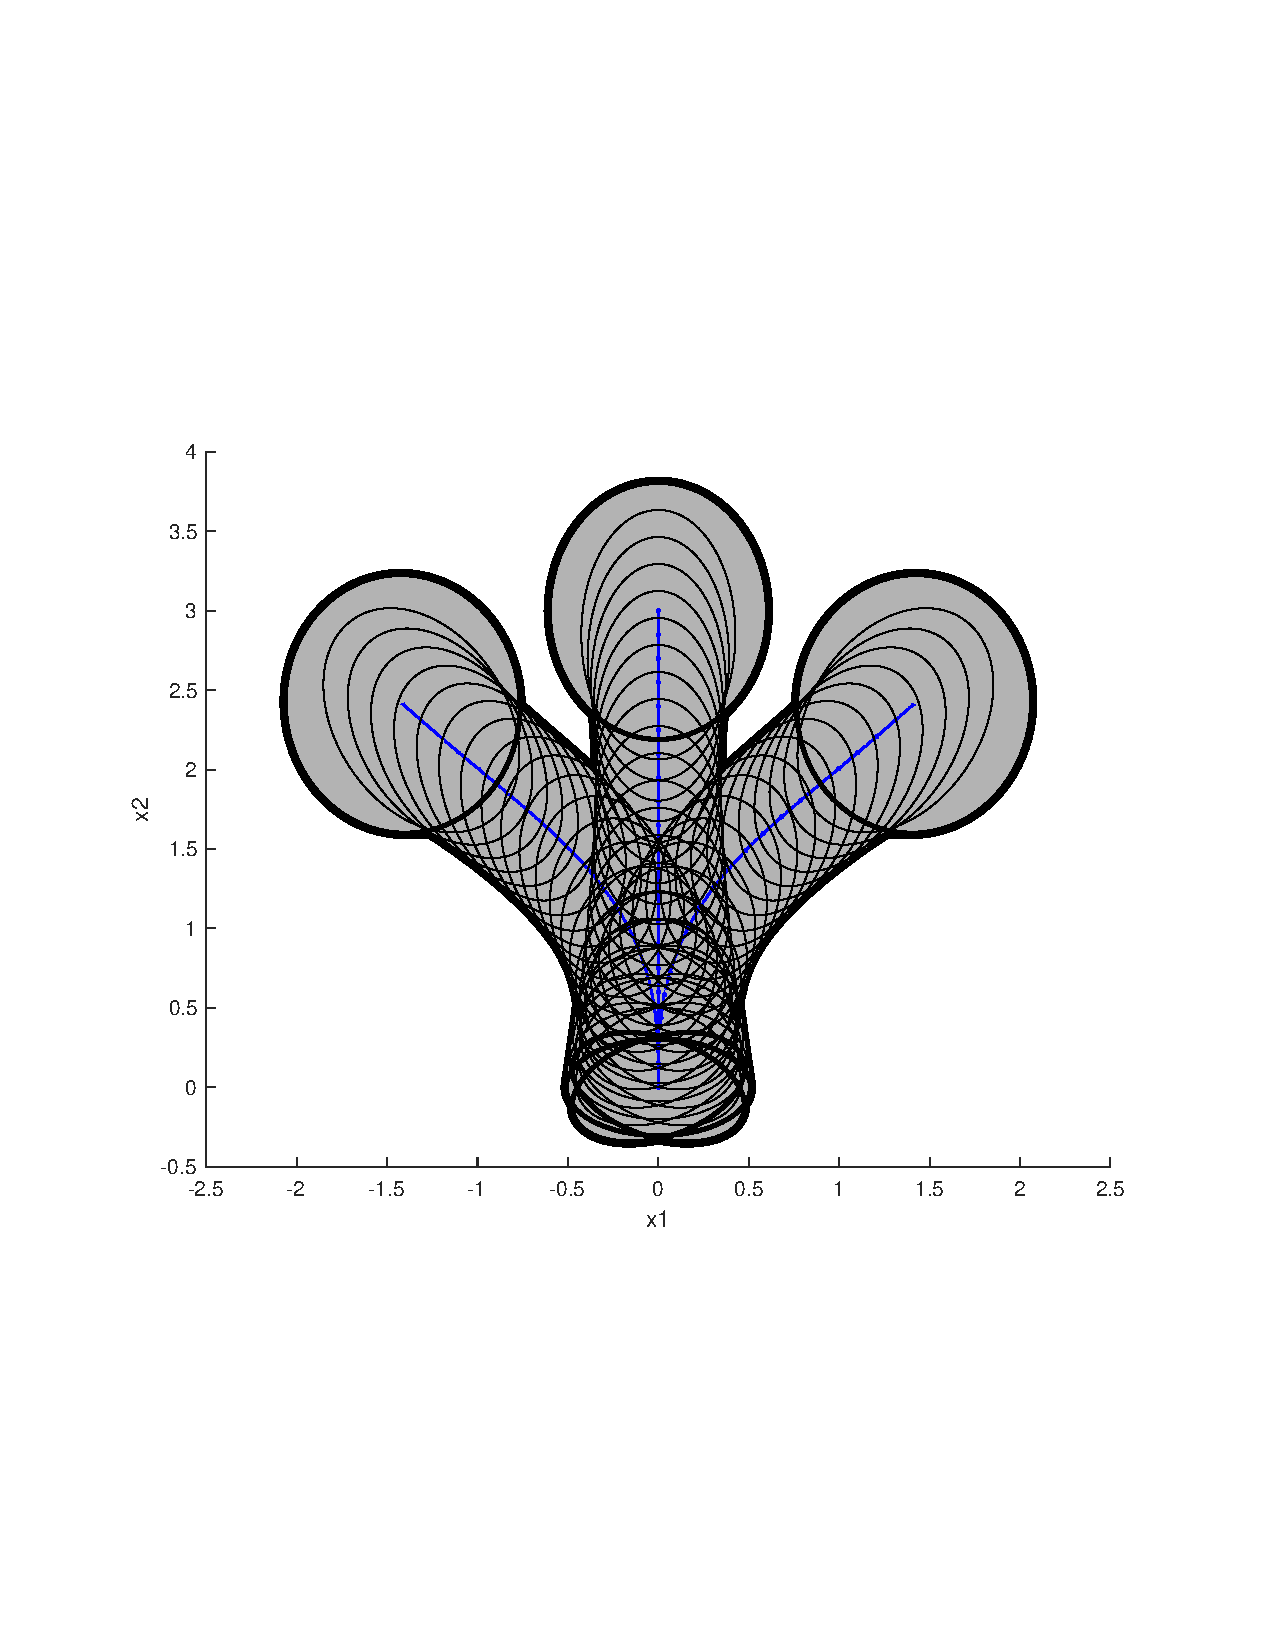
\includegraphics[scale=.5]{figures/experiments/sample-funnel-overlay}
  \caption{Three funnels from the initial trajectories with the projected
    funnels overlaid.}
  \label{fig:sample-funnel-overlay}
\end{figure}

\subsection{LQR cost matrices}
\label{subsec:lqr-cost}

Although the focus of this thesis is not on fine-tuning the controller, some
amount of effort has to go into getting the cost parameters acceptable, so that
the funnels actually converge. In general the strategy is penalizing the
vehicle's distance from the nominal path in \((x,y,\theta)\), and not caring for
the energy expended by the control input. Thus path divergence is penalized
hard, and input divergence is not.

More specifically the cost matrices employed are
\begin{align*}
  R &= 0.01 \\
  Q &= \begin{bmatrix}
    40 & 0 & 0 & 0 \\
    0 & 40 & 0 & 0 \\
    0 & 0 & 40 & 0 \\
    0 & 0 & 0 & 4 \\
  \end{bmatrix}
  \\
  Q_{f} &=
          2\times
          \begin{bmatrix}
            1 & 0 & 0 & 0 \\
            0 & 1.5 & 0 & 0 \\
            0 & 0 & 1 & 0 \\
            0 & 0 & 0 & 1 \\
          \end{bmatrix}
  \\
\end{align*}
where the control input is only penalized \(\frac{1}{10}\)th of the other
variables.

\subsection{Making sure that the vehicle stays within the funnels during
  execution}
\label{subsec:check-vehicle-in-funnel}

During the execution of the \rrtfunnel{} algorithm the planner keeps track of
the funnel during execution, and aborts the simulation with the emergency
maneuver if the vehicle happens to leave one of the funnels at runtime. This
will be counted in the experiments as a collision on the part of the
\rrtfunnel{} algorithm.

\subsection{Show the funnel inlets and outlets from the funnel computations}
\label{subsec:funnel-no-composable}

Unfortunately, the funnels do not compose, and the composition checking of the
algorithm has to be left out. This is because the controller has no influence on
the speed of the vehicle, and hence there is no way to make the system converge
in the direction of speed as exemplified in the~\cref{fig:funnel-conv}.

\begin{figure}
  \centering
  \begin{subfigure}[b]{0.4\textwidth}
    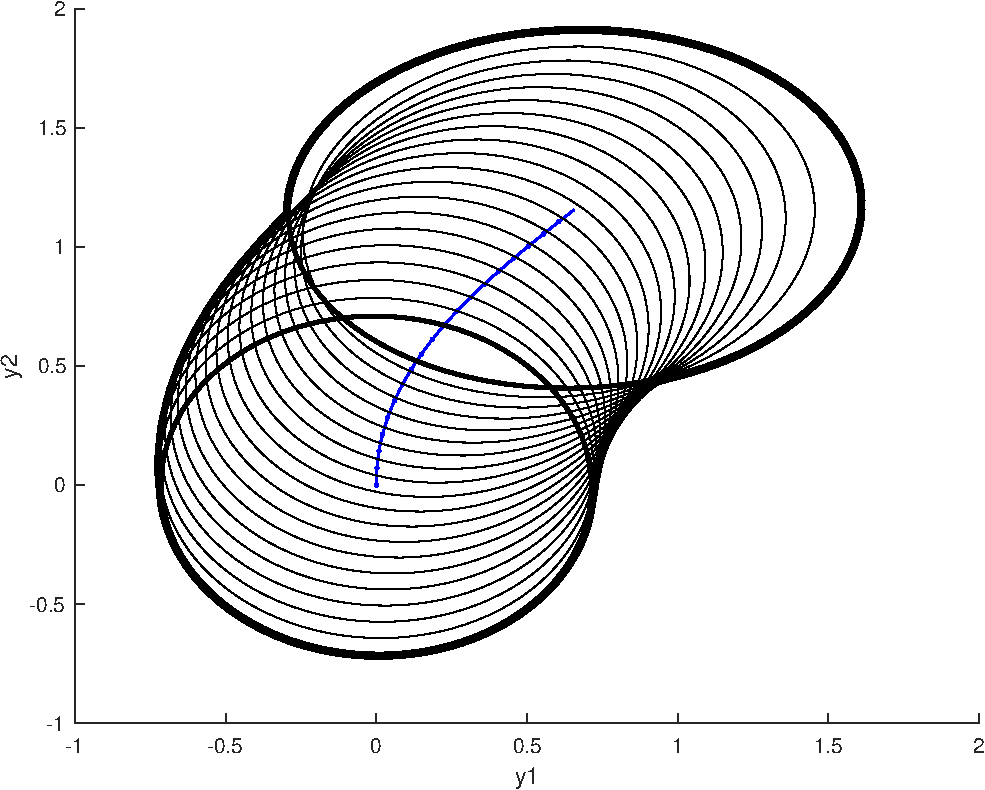
\includegraphics[width=\textwidth]{figures/experiments/sos-calculation}
  \end{subfigure}
  \quad
  \begin{subfigure}[b]{0.4\textwidth}
    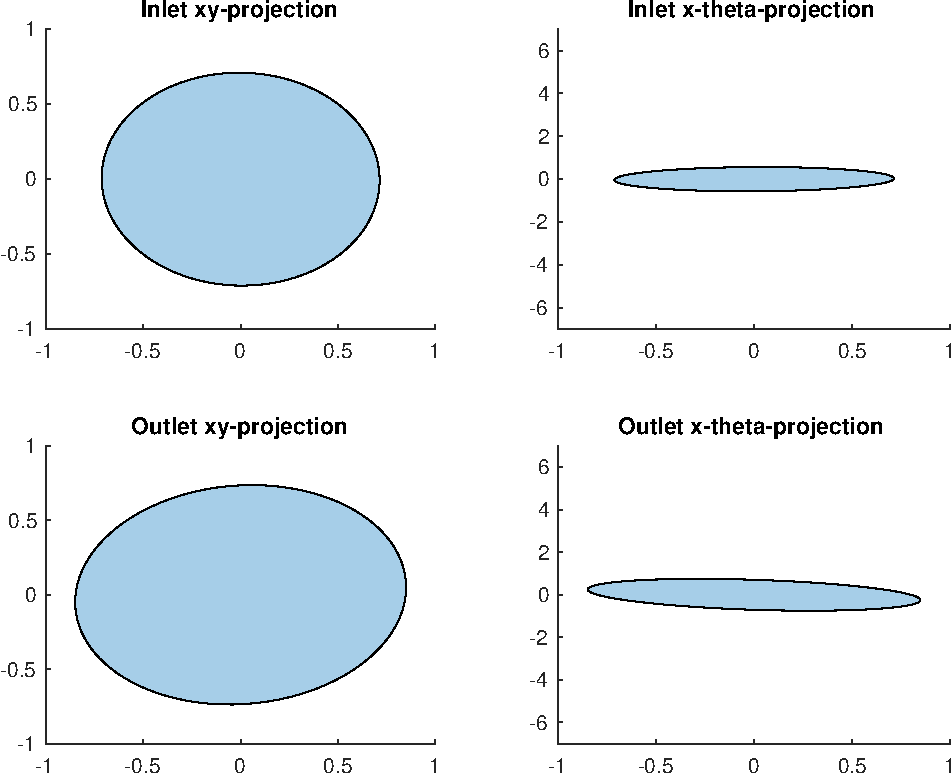
\includegraphics[width=\textwidth]{figures/experiments/sos-calculation-inlet-outlet}
  \end{subfigure}
  \caption{Pictures: A slice of the inlet and the outlet ellipsis in the x-y and
    x-theta dimensions.}
  \label{fig:funnel-conv}
\end{figure}

\section{Experiments}
\label{sec:experiments-final}

The experiments will run the \rrtfunnel{} against a benchmark regular RRT
planner with the motion primitive set pictured
in~\cref{fig:intial-trajectories-exp} on the forest traversal problem pictured
in~\cref{fig:simulated-forest}.

The benchmark-planner is an \ac{RRT} algorithm using the same motion primitive
set as the \rrtfunnel{} algorithm, with the same \ac{LQR} controller, and the
same distance metric. The difference is that it does not take uncertainty into
account, and instead maximizes the distance to the nearest obstacle as the
extension operator \ie{}
\begin{equation}
  \max_{i}\min_{t,j}(x_{i}(t), o_{j})
\end{equation}
where \(x_{i}(t) \in \mathcal{T}\), is a trajectory from the basic motion
primitive set, and \(o_{j} \in \modelobstacle{}\) is an obstacle in the
configuration space \(\modelconfigurationspace{}\).

The end goal is set so that it will not take pose into account, and will only be
concerned with getting within an \(\epsilon\) of the \((x,y)\) in the test map.
For all the experiments below, an \(\epsilon\) of 5\si{\metre} is given to the
planners.

Each test-run will be run in a forest generated with the \textit{Poisson
  process} method from~\nameref{sec:Poisson-Process}, and an intensity parameter
(\(\lambda = 0.1\)), which should yield a pretty dense forest, and hence make
collisions more likely to happen.

The experiments will record the number of collisions for each algorithm across
all test-runs, and the distance penalty obtained total (which is the distance
from the target, if the planner failed to make it there). The planners will run
in the same environment for each test, with the same initial seed, but the
environments will be different for each run, as the Poisson process generating
the obstacle forest is random in nature. With this test setup the difference
between a planner which takes into account uncertainty should become evident.

Before the experiments are run all individual funnels in the base set are run
with a hundred simulations runs from random starting positions in its inlet, to
check if the invariant holds, and that the vehicle stays within the funnel at
all times. This, along with the check whether or not funnels are composable, as
in~\nameref{sec:composable-funnels}, then the invariant that the vehicle never
leaves multiple funnels composed holds.

Uncertainty is added in terms of additive noise with \(w = -0.3\)\si{m.s^{-1}}
in the world x-direction, which is supposed to represent a broken sensor with a
constant drift.

Below are the results from a hundred test-runs with the test setup from above:

\subsubsection{Uncertainty in input}
Model:
\begin{equation}
  \label{eq:model-dynamics-experiments}
  \mathbf{x} =
  \begin{bmatrix}
    x \\ y \\ \theta \\ \dot{\theta} \\
  \end{bmatrix}, \, \dot{\mathbf{x}} =
  \begin{bmatrix}
    -v(t)   \sin(\theta) \\
    v(t) \cos(\theta) \\
    \dot{\theta} \\
    u \\
  \end{bmatrix}
  +
  \begin{bmatrix}
    w \\
    0 \\
    0 \\
    0 \\
  \end{bmatrix}
\end{equation}

What happens if we add more uncertainty than what is modeled? - Run a simple
experiment, to check the robustness of both benchmark algorithms to unmodelled
noise.

TODO - run the experiments with increasing uncertainty, and add this as bar
plots for the experiments with groups of bars for each uncertainty addition.
Then the benchmark planner must not collide without uncertainty!

\begin{figure}
  \centering 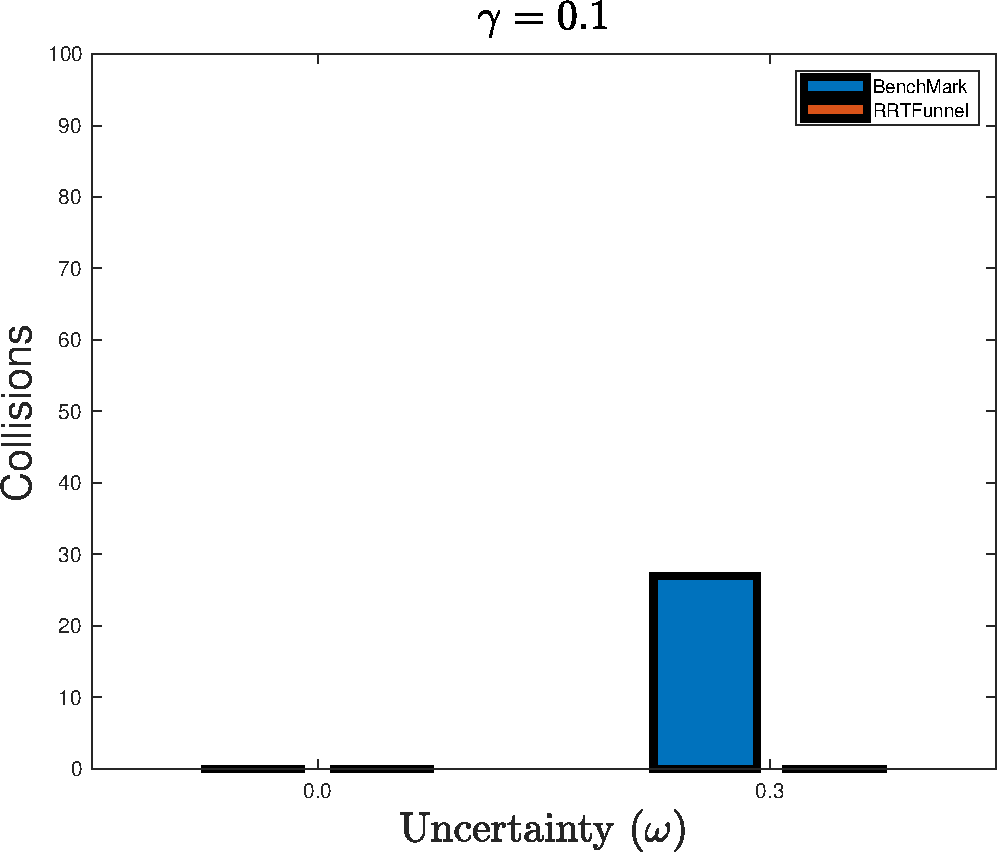
\includegraphics[scale=.5]{figures/experiments/ResultPlot01}
  \caption{Results for forest density = 0.1}
  \label{fig:result0.1}
\end{figure}

\begin{figure}
  \centering \fbox{%
    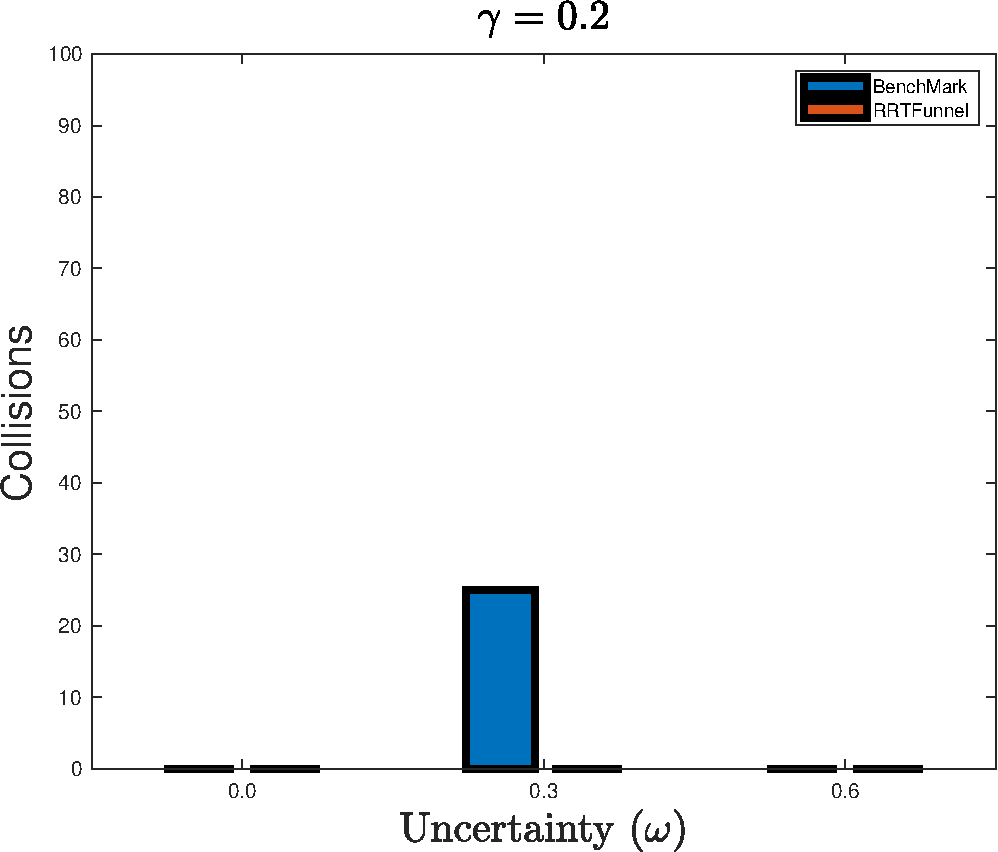
\includegraphics[scale=.5]{figures/experiments/ResultPlot02}}
  \caption{Results for forest density = 0.2}
  \label{fig:result0.2}
\end{figure}
